For the reproducibility purpose, the MATLAB code and datasets used to produce the numerical results in this section are available online at \url{https://github.com/AdMeynard/BoundaryEffectsReduction}.

\subsection{Evaluation the forecasting performance}
In that section, we first evaluate the quality of the forecasting step and compare it the the theoretical results provided by Theorem~\ref{th:error}. The level of the forecasting error depends on at least two parameters:
\begin{itemize}
\item The noise variance $\sigma^2$.
\item The size of the training dataset $K$. 
\end{itemize}
In subsections~\ref{ssse:res.sine} and~\ref{ssse:res.ahm}, we study the influence of these parameters. A comparison with the theoretical results of section~\ref{se:theoretical} is also available.

\subsubsection{Sum of sine waves}
\label{ssse:res.sine}
We proved that the linear dynamic model is sufficient to catch the dynamical behavior of signals taking the form~\eqref{eq:sum.sine}. In order to validate this theoretical result, we apply the forecasting Algorithm~\ref{alg:extension} to a large number of realizations of the random vector $\bx$ following the model~\eqref{eq:model.noise}, and such that the deterministic component $\bz$ takes the form:
\[
\bz[n]\! =\!\cos\!\left(2\pi p_1 \dfrac{n}{M} \right)\! +\! R\cos\!\left(2\pi p_2 \dfrac{n}{M} \right),\quad \!\forall n\!\in\!\{1,\ldots,N\},
\]
with $N=10^4$, $M=150$, $p_1=10$, $p_2=33$ and $R=1.4$. Besides, the additive noise is chosen to be Gaussian: $\bw\sim\cN(\bzero,\bI)$.

\paragraph{Influence of the noise variance $\sigma^2$} Here, the size of the training dataset is set to $K=450$. Then, the forecasting algorithm is run on $1000$ realizations on the discrete signal $\bx$ for three different values of $\sigma$, logarithmically equi-spaced from $10^{-3}$ to $10^{-1}$. For each of these values, we determine the experimental bias, denoted as $\mu_{\xp}[N-1+\ell]$, and experimental variance, denoted as $\gamma_{\xp}[N-1+\ell,N-1+\ell]$, in function of the forecasting sample index $\ell$ (going from $1$ to $L=100$).

The experimental results show that the bias is neither depending on the noise variance $\sigma^2$ nor the forecasting length $\ell$. Indeed, independently of $\sigma$, we always have $\mu_{\xp}[N-1+\ell]\in\left[-0.03\sigma,0.03\sigma\right]$, which is negligible with respect to the magnitude of $\bz$. This result confirms the theoretical result~\eqref{eq:mean.error}. 

On Fig.~\ref{fig:res.noise.sine}, we display the experimental variance $\gamma_{\xp}[N-1+\ell,N-1+\ell]$ for each value of $\sigma$. The associated theoretical asymptotic forecasting variance~\eqref{eq:cov.error.2} is also displayed in solid line. As expected, this result highlights the fact that the forecasting variance increases linearly with respect to $\sigma^2$. Surprisingly, this result shows that the forecasting variance {\em slightly} decreases with $\ell$, what is counterintuitive. 
%
%{\color{red} [HT: need a more convincing explanation.] } 
%It should be noted that, contrary to what expression~\eqref{eq:cov.error.2} suggests, smaller values of $\sigma$ do not cause a decrease of the experimental variance, but an increase. This comes from the fact that when $\sigma$ is small, the matrix $\bX\bX^T$ becomes ill-conditioned. The calculation of the forecasting matrix $\tilde\bA$ in~\eqref{eq:lse} is then strongly disturbed.

\begin{figure}
%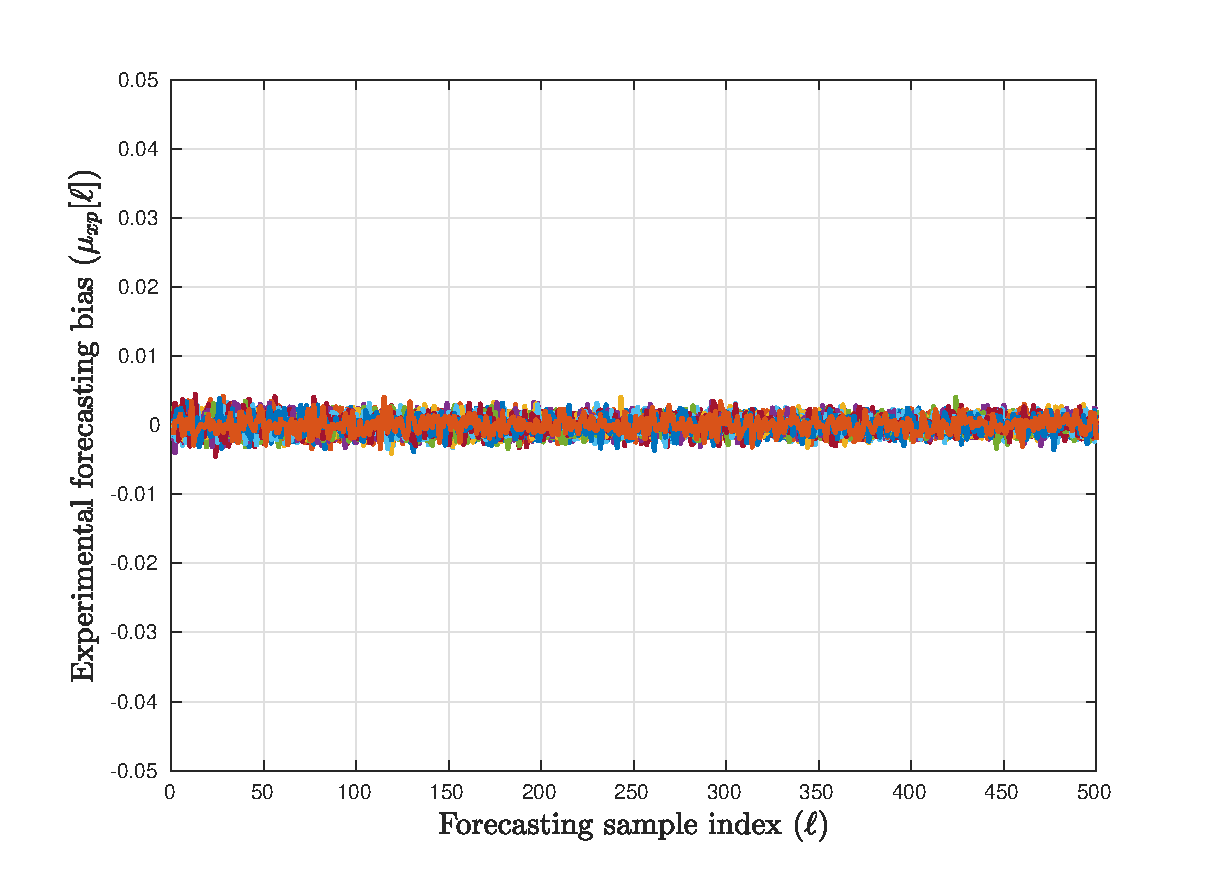
\includegraphics[width=.24\textwidth]{biasNoiseSine.eps}
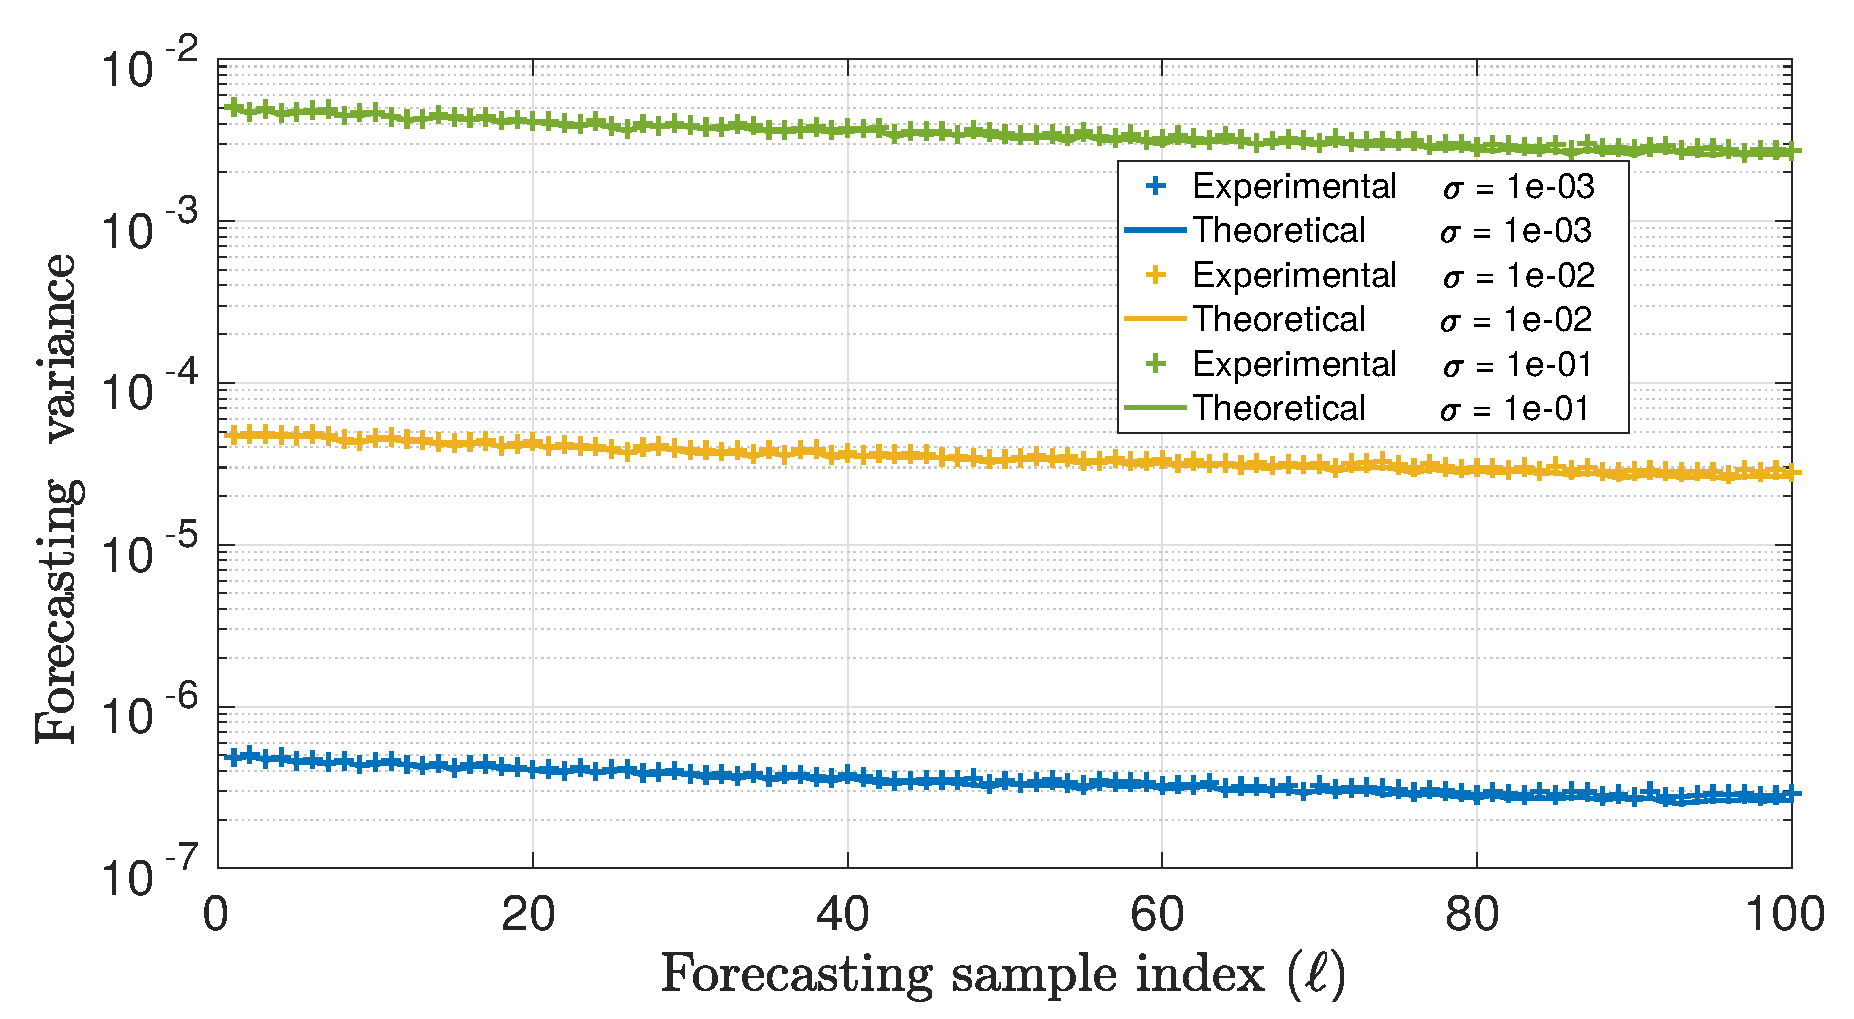
\includegraphics[width=.48\textwidth]{VarianceNoiseSine.eps}
\caption{Evolution of the experimental and theoretical forecasting variance in function of the forecasting sample index for different values of $\sigma$.}
\label{fig:res.noise.sine}
\end{figure}

\paragraph{Influence of the training dataset size $K$} Here, the noise variance $\sigma$ is set to $\sigma=10^{-2}$. Then, the forecasting algorithm is run on 3000 realizations on the discrete signal $\bx$ for three different values of $K$, logarithmically equi-spaced from $4.5\times 10^{2}$ to $2\times 10^{3}$. For each of these values, we determine the experimental bias $\mu_{\xp}[N-1+\ell]$ and variance $\gamma_{\xp}[N-1+\ell,N-1+\ell]$ in function of the forecasting sample index $\ell$ (going from $1$ to $500$). 

As in the previous study, the experimental bias vanishes when $K$ increases, what confirms the approximation result~\eqref{eq:mean.error}. Besides, the experimental variance  is displayed on Fig.~\ref{fig:res.size.sine}, and compared with the associated theoretical variance~\eqref{eq:cov.error.2}. Each color corresponds to these experimental results obtained for a given value of $K$. This result validates the asymptotic behavior provided by~\eqref{eq:cov.error.2}, and we can show that the second order moment $\gamma[\ell,\ell]$ is less dependent on $K$ when $K$ is large.


\begin{figure}
%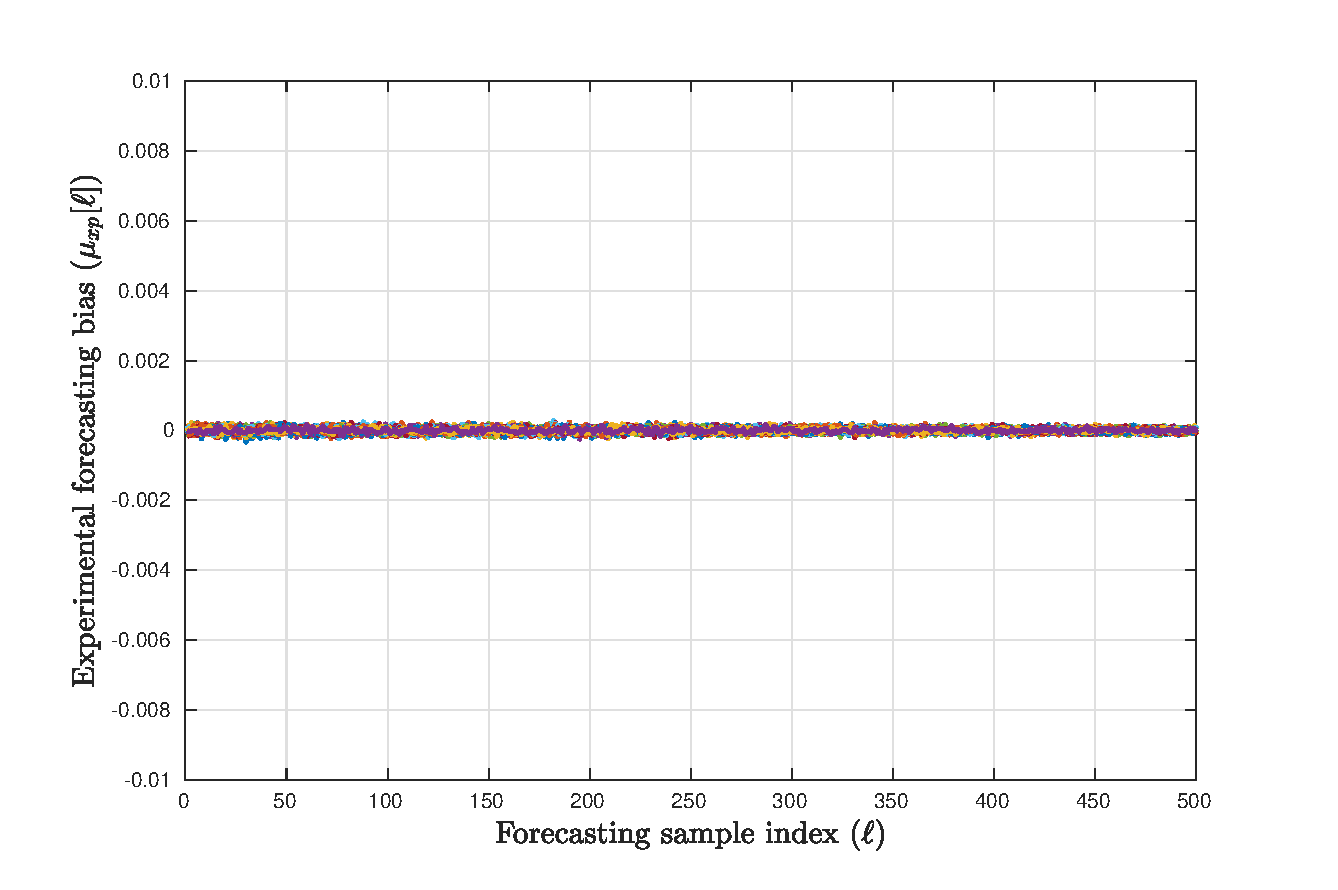
\includegraphics[width=.24\textwidth]{BiasKSine.eps}
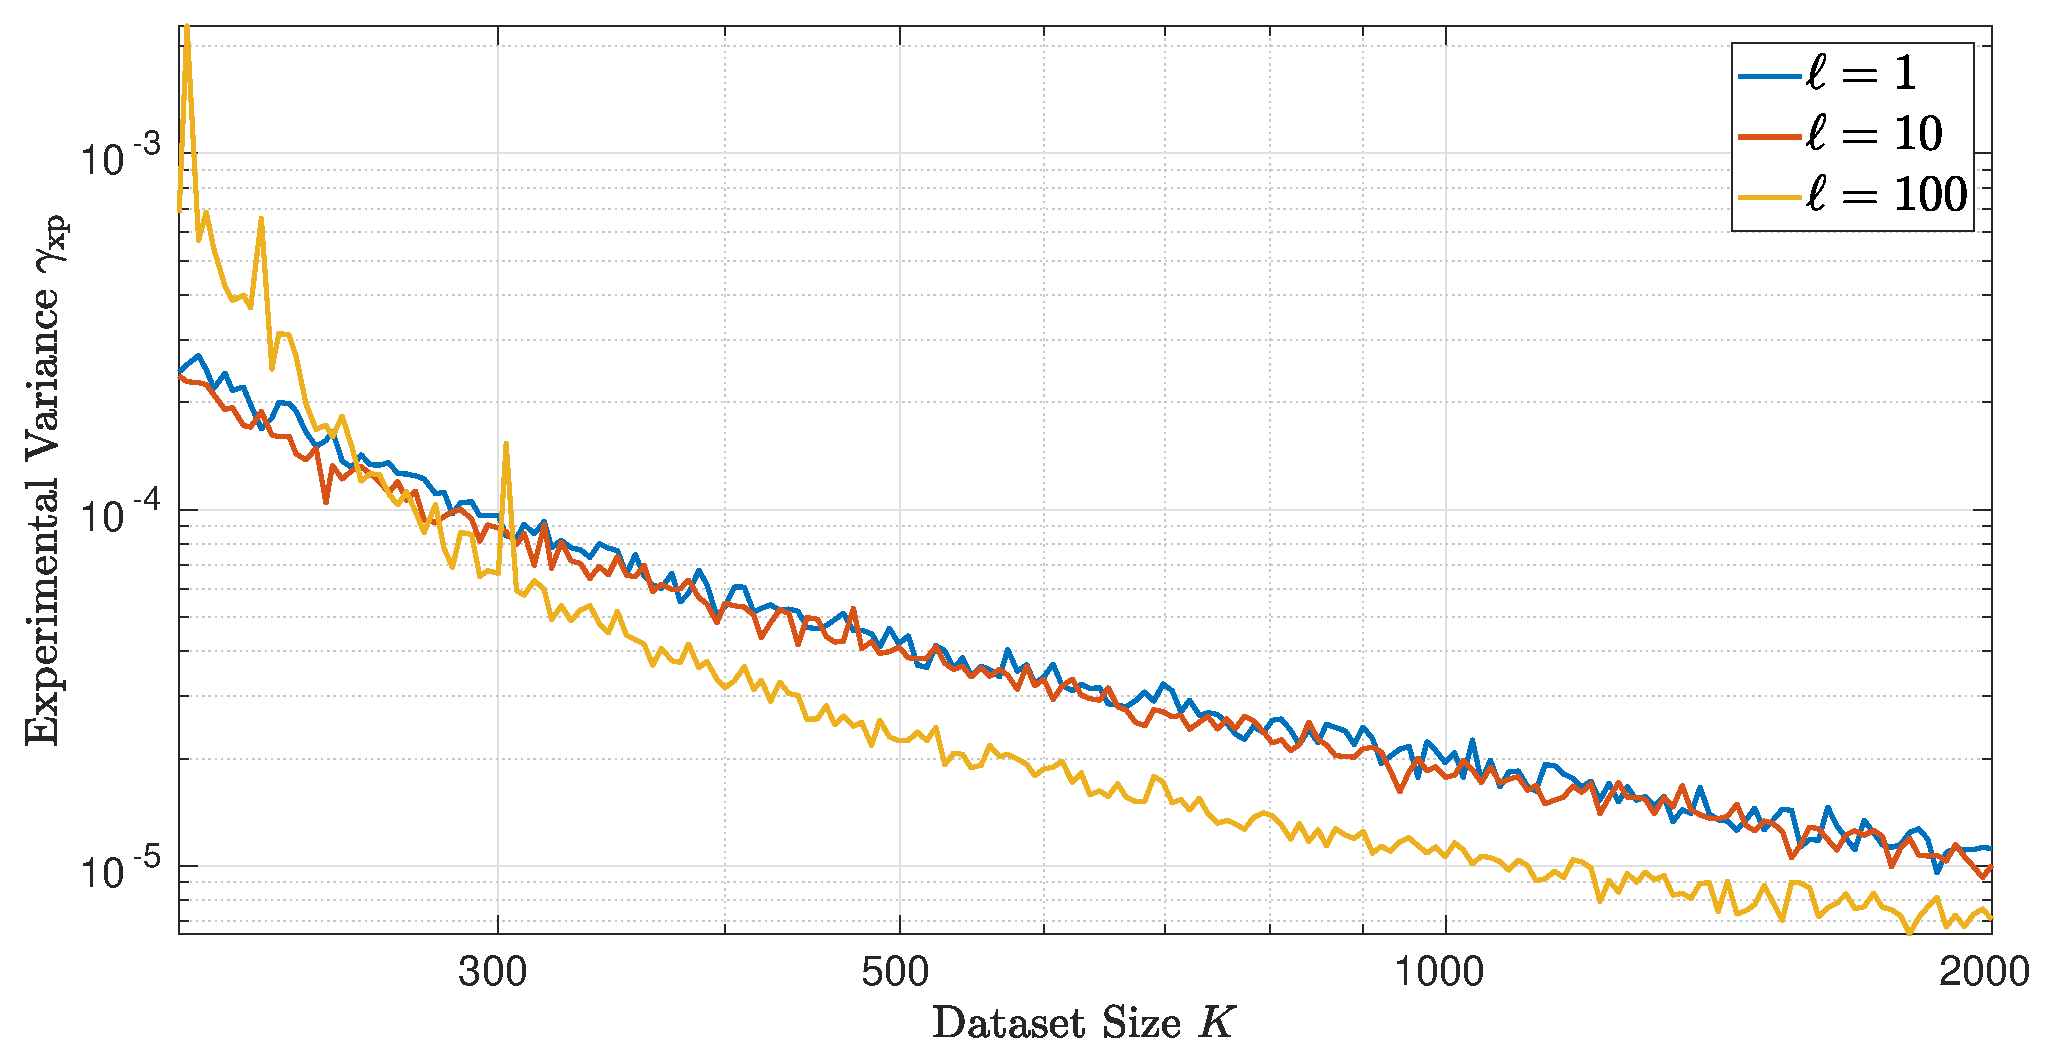
\includegraphics[width=.48\textwidth]{VarianceKSine.eps}
\caption{Evolution of the experimental and theoretical forecasting variance in function of the forecasting sample index for different values of $K$.}
\label{fig:res.size.sine}
\end{figure}

\paragraph{Summary}
Both previous experimental results combined with the theoretical asymptotic equation~\eqref{eq:cov.error.2} allow us to describe the influence of the noise variance and the size of the training dataset on the variance of the forecasting noise, empirically summarized as follows:
\begin{equation}
\gamma[N-1+\ell,N-1+\ell] \underset{K\to\infty}{\approx} \dfrac{\sigma^2}{K}g[\ell] .
\end{equation} 
where $g$ is a bounded positive function. The empirical result is coherent with the theoretical result provided by Theorem~\ref{th:error}.

This study neglects the analysis of the influence of the parameter $M$, whose influence on the value of the experimental variance is numerically not significant as long as $M\ll 2K$. The choice of this parameter is especially crucial when the deterministic component of the signal is no longer stationary. The AHM, discussed below, is an example.

\subsubsection{Adaptive harmonic model}
\label{ssse:res.ahm}
We now consider a signal satisfying the AHM so that the instantaneous frequencies and amplitudes of its components vary over time. The deterministic component $\bz$ of the random vector $\bx$ (constructed following the model~\eqref{eq:model.noise}) takes the following form, for all $n\in\{1,\ldots,N\}$:
\[
\bx[n] = \cos\left(2\pi \phi_1[n] \right) + R[n]\cos\left(2\pi \phi_2[n] \right) \ ,
\] 
where the instantaneous amplitude $R$ is given by:
\[
R[n] = 1.4 + 0.2\cos\left(4\pi\frac{n}{N}\right)\ ,
\]
and the instantaneous phases are such that:
\begin{align*}
\phi_1[n] &= \frac{p_1}{M}\left( n + \frac{0.01}{2\pi}\cos\left(2\pi\frac{n}{N}\right) \right) \\[-1mm]
\phi_2[n] & = p_2\frac{n}{M} + \frac{20}{2N\fs}n^2
\end{align*}
Besides, the noise is chosen to be Gaussian: $\bw\sim\cN(\bzero,\bI)$, and we take: $N=10^4$, $M=750$, $p_1=10$, $p_2=23$.

To highlight the fact that the linear dynamical model is sufficient to catch most of the dynamical behavior of signals following the AHM, we compare the performance of the Algorithm~\ref{alg:boundary} with a simple extension obtained by pointwise symmetrization~\cite{Kharitonenko02wavelet}. We also evaluate the performance of reference forecasting algorithm that could be used for extending such signals. These methods are:
\begin{itemize}
\item The EDMD has been developed by Williams \etal~\cite{Williams15data}. The proposed algorithm is a way to obtain an approximation of the so-called Koopman operator of the observed system, which theoretically allows to catch dynamic of nonlinear systems~\cite{Korda18linear}.
\item The GPR~\cite{Rasmussen06gaussian} is a method relying on a probabilistic dynamical model. That one is based on the Gaussian process structure, and therefore offer more flexibility in the type of dynamic that could be modeled than the linear model~\eqref{eq:dyn.model}.
\item The TBATS method~\cite{DeLivera11forecasting} is based on a classical decomposition of times series into a trend, a seasonal and an ARMA components, with a specific dynamic for the seasonal component. This model demands the estimation of numerous parameters and, by implication, may be slow. 
\end{itemize}

To quantify the global quality (\ie~not depending on $\ell$) of the forecasting approaches, we evaluate the Experimental Mean Square Error $\mathrm{MSE_{xp}}(\tilde\bx)$ of the forward forecast extended signals, namely:
\begin{align}
\label{eq:mse}
\mathrm{MSE_{\xp}}(\tilde\bx) &= \dfrac1{L}\|\tilde\bx -\bx^\mathrm{ext}\|^2 \\[-1mm]
\nonumber
&=\! \dfrac1{L}\sum_{\ell=1}^L \bmu_{\xp}[N\!-\!1\!+\!\ell]^2 \!+\! \bgamma_{\xp}[N\!-\!1\!+\!\ell,N\!-\!1\!+\!\ell] .
\end{align}
where $\bx^\mathrm{ext}$ is the ground-truth extended signal, that is: $\bx^\mathrm{ext} = \begin{pmatrix}\bx[-L] & \cdots & \bx[N-1+L] \end{pmatrix}$. Then, as long as the bias $\bmu[N-1+\ell]$ and the variance $\bgamma[N-1+\ell,N-1+\ell]$ of the forecasting estimator remain small for all $\ell$, the MSE takes small values either. Corresponding results are given in Table~\ref{tab:mse.sine}. They show that the naive extension we propose gives satisfying results, in particular in comparison with the point-symmetric extension. Besides, even though the other more sophisticated methods, like GPR, give MSE values that have a slightly smaller standard deviation, these methods are substantially limited by the computing time they require, which prevent them from being used to exploit real-time data. Thus, {\sf SigExt} is the extension method that optimize the trade-off between the forecasting quality and the computing time. %That is why, it is implemented in our algorithm for the reduction of boundary effects.

\begin{table}
\centering
\caption{AHM signal: performance of the extension methods.}
\begin{tabular}{|c||c|c|c|}
  \hline
   \multirow{2}{40pt}{\centering Extension method} & \multicolumn{2}{c|}{MSE}  & \multirow{2}{41pt}{Computing time (sec.)} \\
   \cline{2-3} & Mean & Standard deviation & \\
   \hhline{|=#=|=|=|}
   {\sf SigExt} & $1.433\times 10^{-3}$ & $4.361\times 10^{-4}$ & $0.152$ \\
   \hline
   Symmetric & $1.019\times 10^{1}$ & $1.192\times 10^{2}$ & $0.002$ \\
   \hline
   EDMD & $3.076\times 10^{-2}$ & $8.095\times 10^{-2}$ & $2.537$\\
   \hline
   GPR & $1.436\times 10^{-3}$ & $4.346\times 10^{-4}$ & $146.331$ \\
   \hline
   TBATS & $1.732\times 10^{-3}$ & $4.924\times 10^{-4}$ & $1837.120$ \\
   \hline
\end{tabular}
\label{tab:mse.sine}
\end{table} 


\subsection{Evaluation of the quality of the boundary effects reduction}

\subsubsection{Metrics}
The quality of the boundary effects reduction is evaluated directly on the TF representation. To that aim, we compare the obtained representation to the optimal representation $\ccF_N^\mathrm{opt}(\bx)$, defined as the restriction of the representation of the ground-truth extended signal $\bx^\mathrm{ext}$. Therefore, we have:
\begin{equation}
\ccF^\mathrm{opt}(\bx_N) = \cR\left( \ccF(\bx^\mathrm{ext}) \right) \ .
\label{eq:opt.TFR}
\end{equation} 

In the aim of comparing the different techniques, we use a criterion, proposed in~\cite{Daubechies16conceft}, that quantify the distance between a given TF representation and the optimal one. It is built in analogy with the optimal transport distance, which enables quantifying the distance between two probability density functions. Let us generically denote a time frequency representation $\ccQ$. Then, for $t$ fixed, we consider the following probability density function: $p_\ccQ^t(\xi) = \left. |\ccQ(\xi,t)|^2 \middle/ \int_\RR |\ccQ(\nu,t)|^2\dd\nu \right.$. At each instant $t$, we can then determine the optimal transport distance $d_{t}$ between the two densities. It is given by the $L^1$ norm of the difference between the associated distribution functions. In other words, we have:
\begin{equation*}
d_{t}(\ccQ,\ccF_0) = \int_\RR\left|\tilde P_{\ccQ}^t(\xi)-  P_{\ccF_0}^t(\xi)\right|\dd\xi\ ,
\end{equation*}
where $P_{\ccQ}^t(\xi)=\int_{-\infty}^\xi p_{\ccQ}^t(\nu)\dd\nu$ and $\tilde P_{\ccF_0}^t(\xi)=\int_{-\infty}^\xi\tilde p_{\ccF_0}^t(\nu)\dd\nu$. The \textit{Optimal Transport Distance (OTD)} quantifies the proximity between the estimated and actual instantaneous frequencies while favoring the sparsity of the estimated TF representation. That is why, the performance index $D(\ccQ)$ for the reduction of boundary effects of a given TF representation $\ccQ$ is given by the ratio between its averaged OTD to the optimal TF representation $\ccF^\mathrm{opt}$ (see~\eqref{eq:opt.TFR}) and the averaged OTD of the original TF representation $\ccF$ to $\ccF^\mathrm{opt}$, that is:
%\begin{equation}
%D(\ccQ) = \dfrac1{|I|}\bigintssss_I\ \frac{d_{t}\left(\ccQ,\ccF^\mathrm{opt}\right)}{d_{t}\left(\ccF,\ccF^\mathrm{opt}\right)}\ \dd t\ .
%\label{eq:index.perf}
%\end{equation}
\begin{equation}
D(\ccQ) = \dfrac{\displaystyle\int_I d_{t}\left(\ccQ,\ccF^\mathrm{opt}\right)\dd t}{\displaystyle\int_I d_{t}\left(\ccF,\ccF^\mathrm{opt}\right)\dd t}\ .
\label{eq:index.perf}
\end{equation}
Thus, $D(\ccQ)<1$ means a reduction of the boundary effects. Let us evaluate the quality of the boundary effects reduction on biomedical signals.


\subsubsection{Respiratory signal}
We first consider a respiratory signal of 6 hours 20 minutes. This signal, a small portion of which is displayed in Fig.~\ref{fig:tho}, is sampled at $\fs=100$~Hz.

\begin{figure}
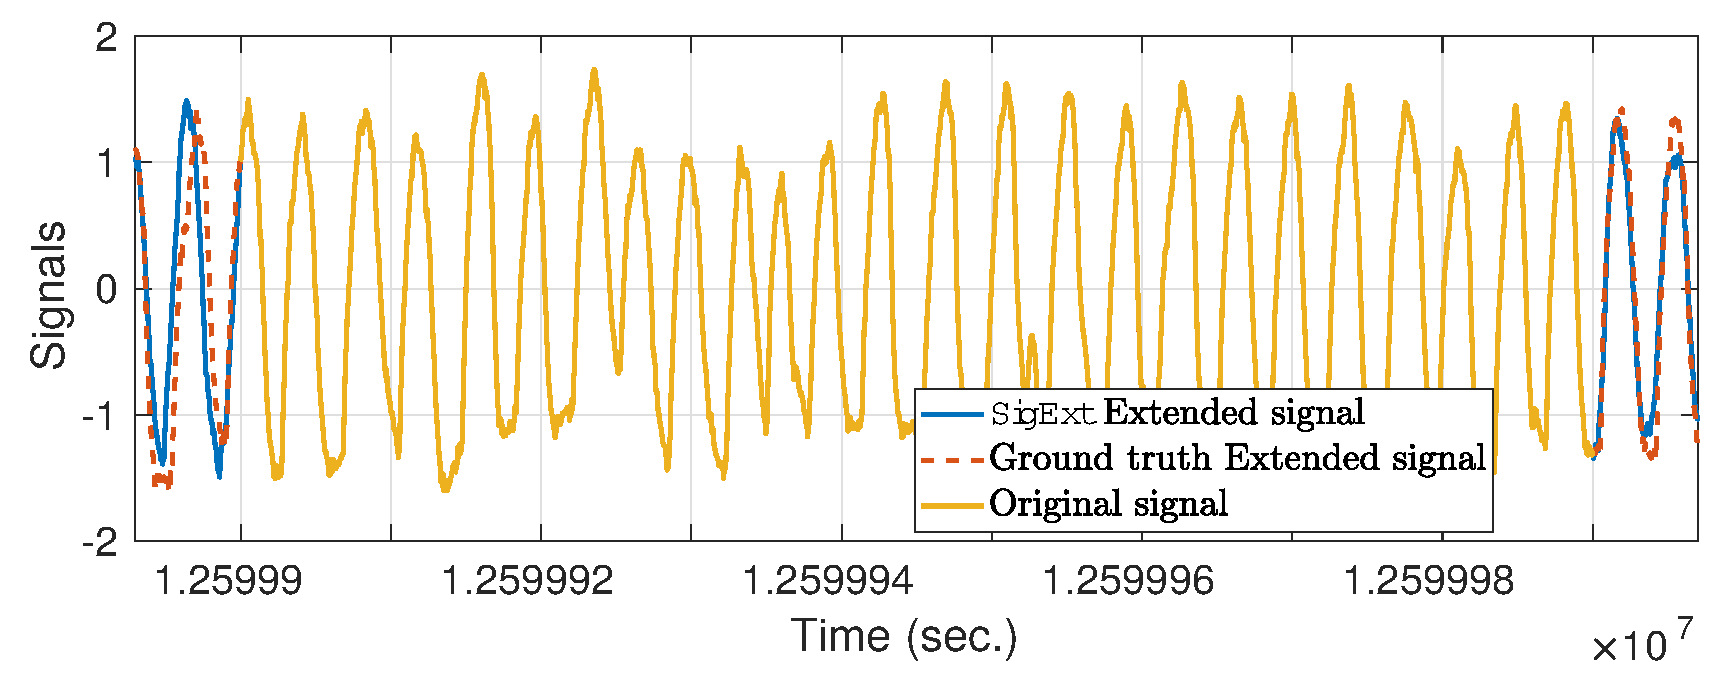
\includegraphics[width=.48\textwidth]{THOforecast.eps}
\caption{Extended THO signal (blue) obtained by the {\sf SigExt} forecasting (top), the EDMD forecasting (middle), and the GPR forecasting (bottom), superimposed with the ground truth signal (red dash).}
\label{fig:tho}
\end{figure}

From that large signal, we build a dataset of $378$ non-overlapping signals of 60 seconds, \ie~$N=6000$. On each of these pieces of signal, we implement the forecasting method introduced in section~\ref{ssse:res.ahm}, including the {\sf SigExt} method detailed in Algorithm~\ref{alg:extension}. However, the TBATS extension method in not implemented here because of its excessive computing time. We forecast $7$-second-long extensions on each segment of signal, corresponding to $L =700$. Thus, in order to catch slowly varying dynamical behaviors, the size of the training signal $M$ is chosen so that $M=\lfloor 1.5L\rfloor$. As a result of section~\ref{ssse:res.sine}, we take: $K=\lfloor2.5M\rfloor$. The resulting MSE~\eqref{eq:mse} averaged with respect to the simulations are given in Table~\ref{tab:THO}. The MSE of {\sf SigExt} is higher than the MSE of the other methods. This is mainly caused by the presence of a few segments of the whole signal involving complicated behaviors, that are unpredictable via a too simple dynamical model like~\eqref{eq:dyn.model}. The left of Fig.~\ref{fig:THO.failure} illustrates one of those cases, where {\sf SigExt} fails to catch the fast varying dynamic of the instantaneous amplitude to satisfactorily forecast the signal. The EDMD an Symmetric extensions are more robust to those situations, as shown on this example and in Table~\ref{tab:THO}. Nevertheless, {\sf SigExt} provides a sufficiently relevant extension to give TF representations sparingly affected by boundary effects. On the right of Fig.~\ref{fig:THO.failure}, we display comparison between the right boundary of SST of the same segment of signal (top-right), and its boundary-free SST obtained after the {\sf SigExt} forecasting (bottom-right). The extension of the instantaneous frequency visible on the right side of the image, illustrates the reduction of boundary effects produced despite an inaccurate signal forecasting.

We then apply {\sf BoundEffRed} (\ie~Algorithm~\ref{alg:boundary}) for diverse TF representations: STFT, SST, RS, as well as concentration of frequency and time (ConceFT), a generalized multitaper SST-based representation introduced in~\cite{Daubechies16conceft}. In Table~\ref{tab:THO}, we give the averaged performance index~\eqref{eq:index.perf}, evaluated the whole TF representations (including  boundaries). Even though {\sf SigExt} performs somehow moderately, the boundary effects are dramatically reduced on the TF representations, in the same order of magnitude than with the forecastings given by EDMD or GPR. Notice that the extension length $L$ has been set accordingly to the window length used by the TF analysis tool. For instance, the window length used to evaluate the STFT is of $1500$ samples. To prevent the STFT from being sensitive to the boundaries, we set $L=750$. In this way, the evaluation of the spectral content of the signal near its boundaries is not limited by a lack of information all along the window support. From now on, all results are given for $L$ equal to the half of the width of the window used in the TF transform.

\begin{table}
\centering
\caption{Respiratory signal: Performance of extension methods and associated boundary-free TF representations.}
\begin{tabular}{|c||c||c|c|c|c|}
  \hline
   \multirow{2}{40pt}{\centering Extension method} & \multirow{2}{35pt}{\centering Averaged MSE} & \multicolumn{4}{c|}{Averaged performance index $D$} \\
   \cline{3-6}
      & & STFT & SST & RS & ConceFT \\
   \hhline{|=#=#=|=|=|=|}
   {\sf SigExt} & $0.046$ & $0.698$ &  $0.705$ & $0.694$ & $0.776$ \\
   \hline
   Symmetric & $0.039$ & $0.984$ & $1.280$ & $9.063$ & $1.295$ \\
   \hline
   EDMD & $0.022$ & $0.635$ &  $0.757$ & $0.701$ & $0.793$ \\
   \hline
   GPR & $0.045$ & $0.793$ &  $0.817$ & $0.727$ & $0.876$ \\ 
   \hline
\end{tabular}
\label{tab:THO}
\end{table}

\begin{figure}
\centering
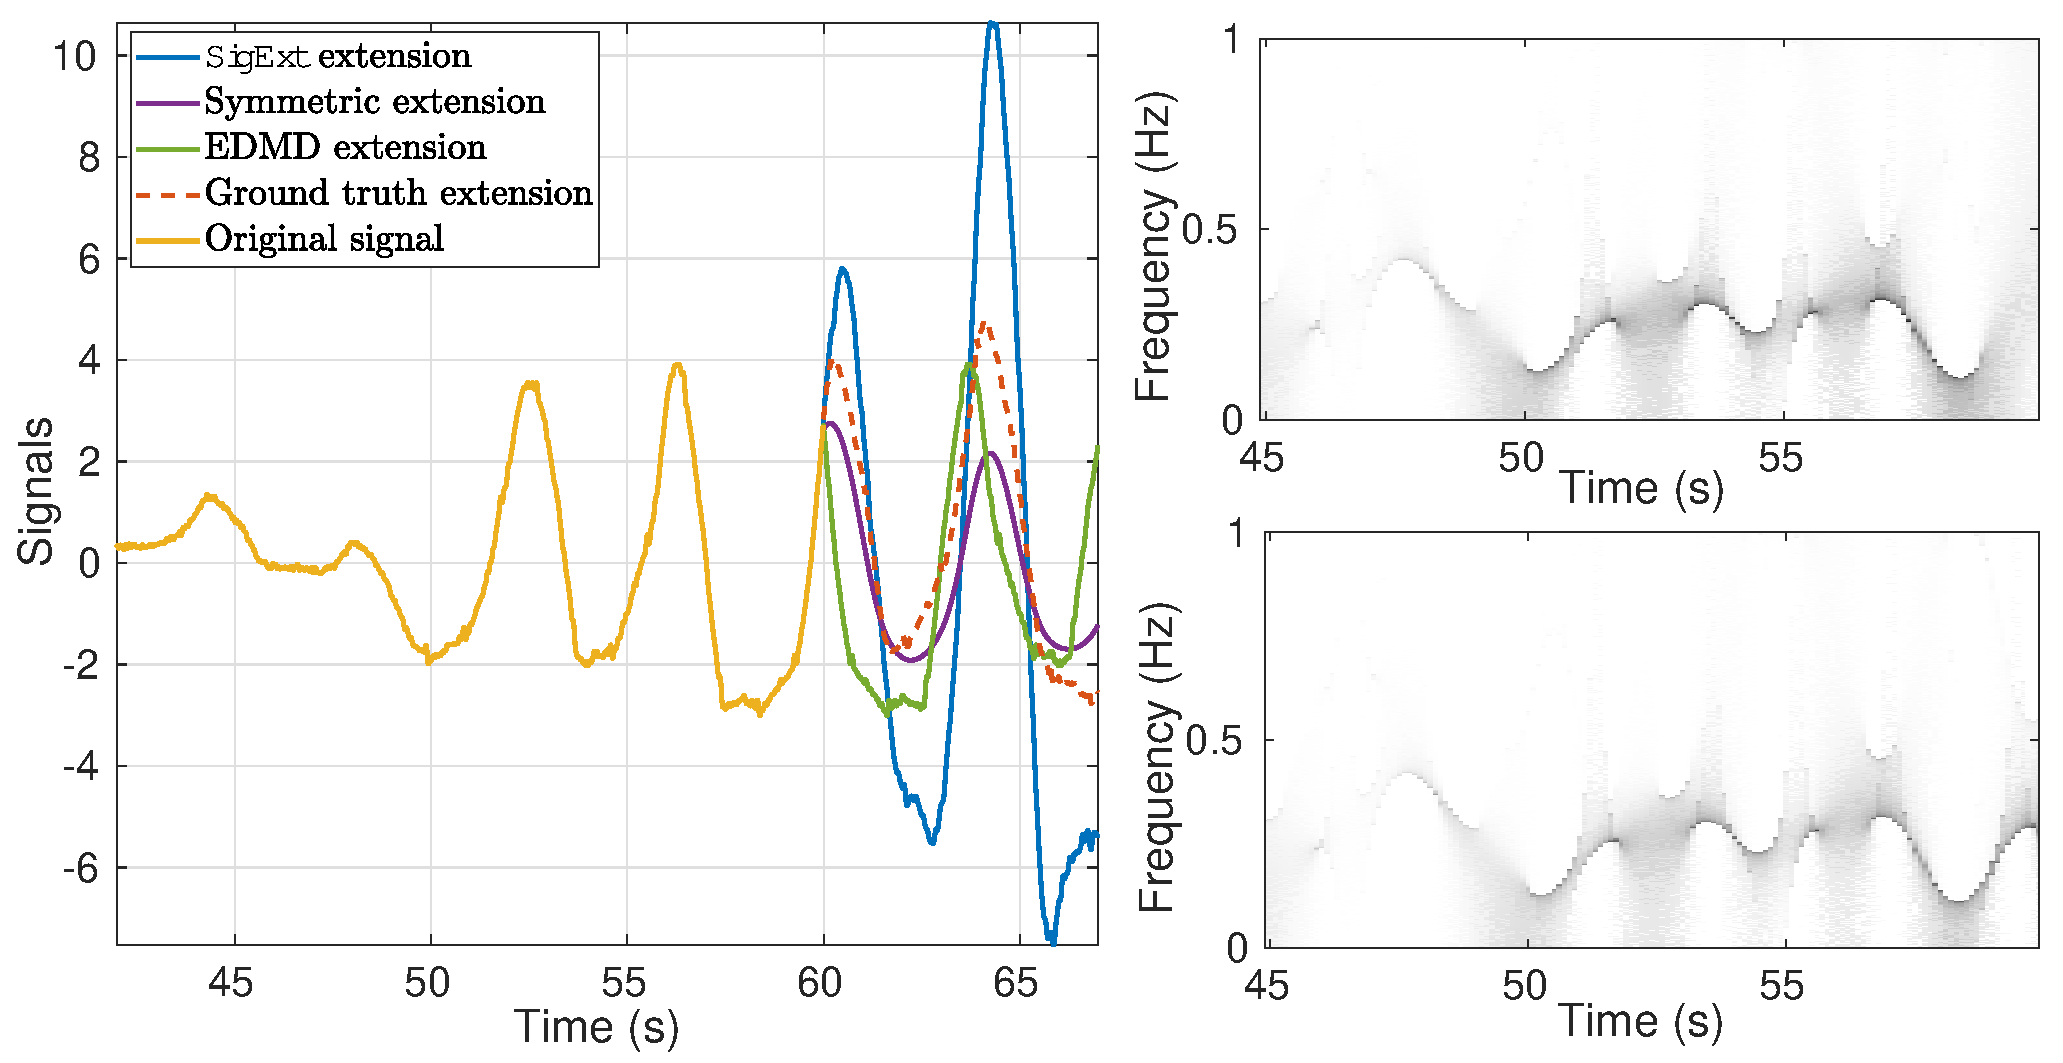
\includegraphics[width=.48\textwidth]{THOfailure.eps}
\caption{Extensions of a segment of the respiratory signal (left) where {\sf SigExt} is outperformed by the EDMD and Symmetric extensions. Corresponding SST (top-right) and boundary-free SST obtained with {\sf SigExt} (bottom-right).}
\label{fig:THO.failure}
\end{figure} 

Finally, in order to verify the ability of {\sf BoundEffRed} to be implemented in real time, we evaluate the computation time required for each iteration of Algorithm~\ref{alg:boundary}, updating of the boundary-free TF representation. This check is performed on the real-time SST of a 10-minute sample of the respiratory signal. As the SST is temporally sub-sampled by a ratio of 20, the update should not exceed $20/\fs=0.2$~sec. This is indeed the case, as no iteration lasted longer than $0.17$ sec on a 6-Core Xeon CPU running at 3.5~GHz and 64~GB of RAM.


\subsubsection{Photoplethysmogram}
\label{ssse:ppg}
We perform a study similar to the previous one on a 640 second-long photoplethysmogram (PPG) signal extracted from the Physionet dataset~\cite{Pimentel17toward, Goldberger00physiobank}, sampled at $\fs=125$~Hz. A portion of this signal is displayed in Fig.~\ref{fig:ppg}. The estimated 5 seconds extensions of this segment obtained by {\sf SigExt}, EDMD and GPR forecastings  are superimposed to the ground-truth extension in Fig.~\ref{fig:ppg}.

\begin{figure}
%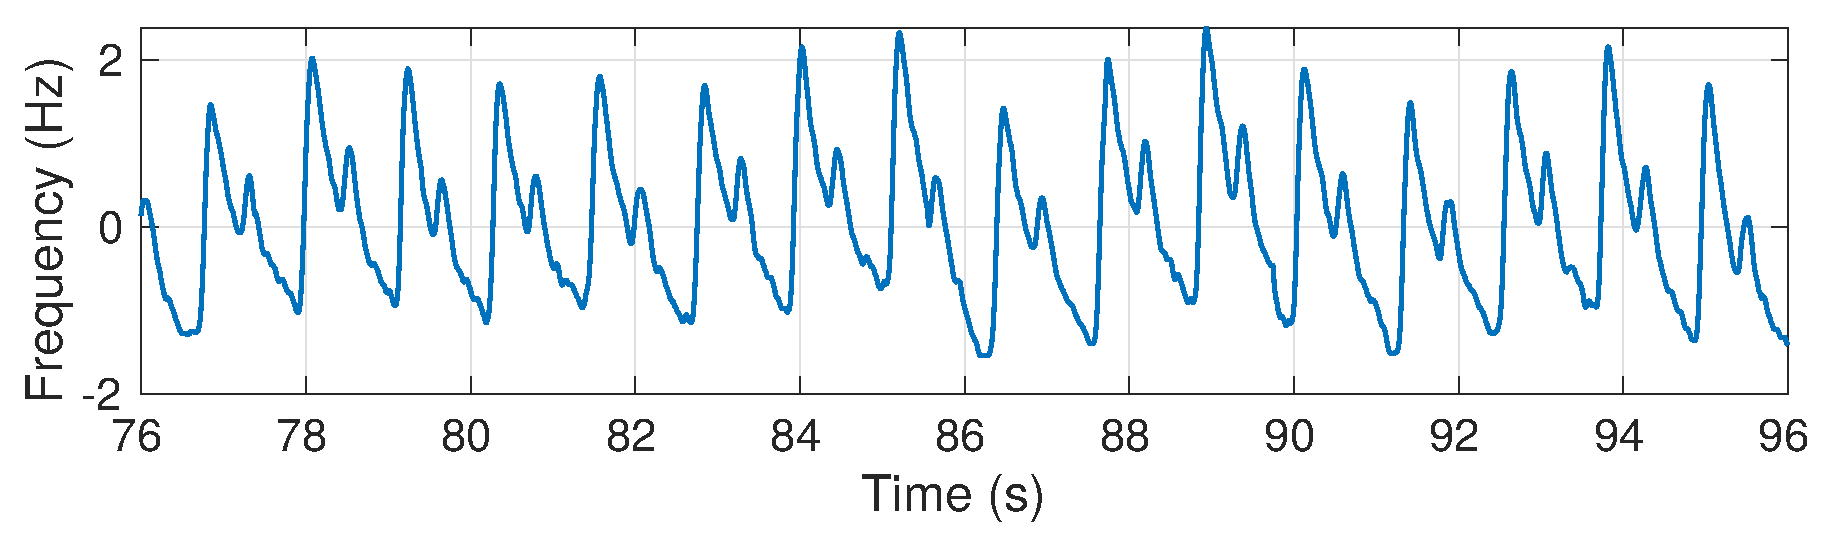
\includegraphics[width=.48\textwidth]{PPGsig.eps}
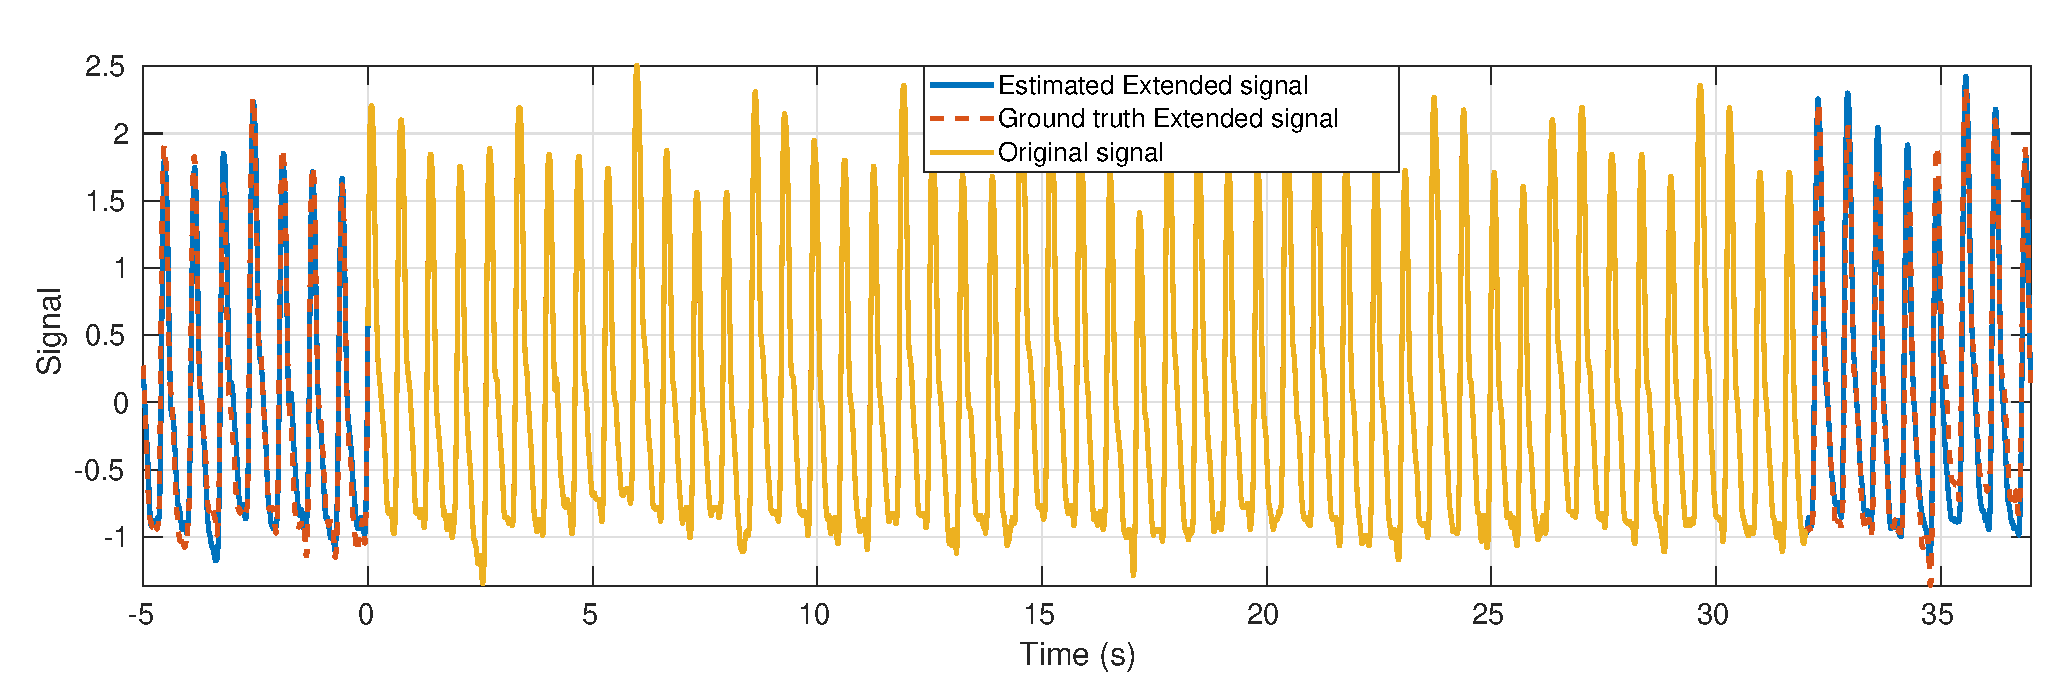
\includegraphics[width=.48\textwidth]{PPGforecast.eps}
\caption{Extended PPG signal (blue) obtained by the {\sf SigExt} forecasting (top), the EDMD forecasting (middle), and the GPR forecasting (bottom), superimposed with the ground truth signal (red dash).}
\label{fig:ppg}
\end{figure}

We divide the signal into 32-second-long segments, and apply Algorithm~\ref{alg:boundary} on each piece. We provide in Table~\ref{tab:otd.ppg} the performance index $D$ of the boundary-free TF representations averaged over the signals. For all the considered TF representations, the results clearly shows that our algorithm reduces the boundary effects. %This highlights the ability of our approach to limit the distortion due the boundary effects and provide a more accurate representations. 
Even though, on this signal, the {\sf SigExt} extension yields TF representations slightly more sensitive to boundary effects than the extensions given by EDMD or GPR, it is the only technique that allows a real-time implementation.

\begin{table}
\centering
\caption{PPG signal: Performance of the boundary-free TF representations according to the extension method.}
\begin{tabular}{|c||c|c|c|}
  \hline
   \multirow{2}{40pt}{\centering Extension method} & \multicolumn{3}{c|}{Averaged performance index $D$} \\
   \cline{2-4}
      & STFT & SST & ConceFT\\
   \hhline{|=#=|=|=|}
%   Without extension & $2.52\times 10^{-2}$ & $9.41\times 10^{-2}$ & $1.03\times 10^{-1}$ \\
%   \hline
   {\sf SigExt} & $0.425$ & $0.713$ & $0.687$ \\
   \hline
   Symmetric & $1.335$ & $1.340$ & $1.258$ \\
   \hline
   EDMD & $0.406$ & $0.642$ & $0.615$ \\
   \hline
   GPR & $0.448$ & $0.766$ & $0.730$ \\
   \hline
\end{tabular}
\label{tab:otd.ppg}
\end{table}

On the bottom-right panel of Fig.~\ref{fig:ex.intro}, we display the SST resulting from the {\sf BoundEffRed} strategy, applied to the portion of PPG displayed on Fig.~\ref{fig:ppg}. We clearly observe an improvement of the quality of the SST near boundaries. Indeed, the blurring visible when zooming on the right boundary of the SST has almost vanished. The real-time tracking of the instantaneous frequencies contained in the measured signal is therefore largely facilitated.

%\begin{figure}
%\centering
%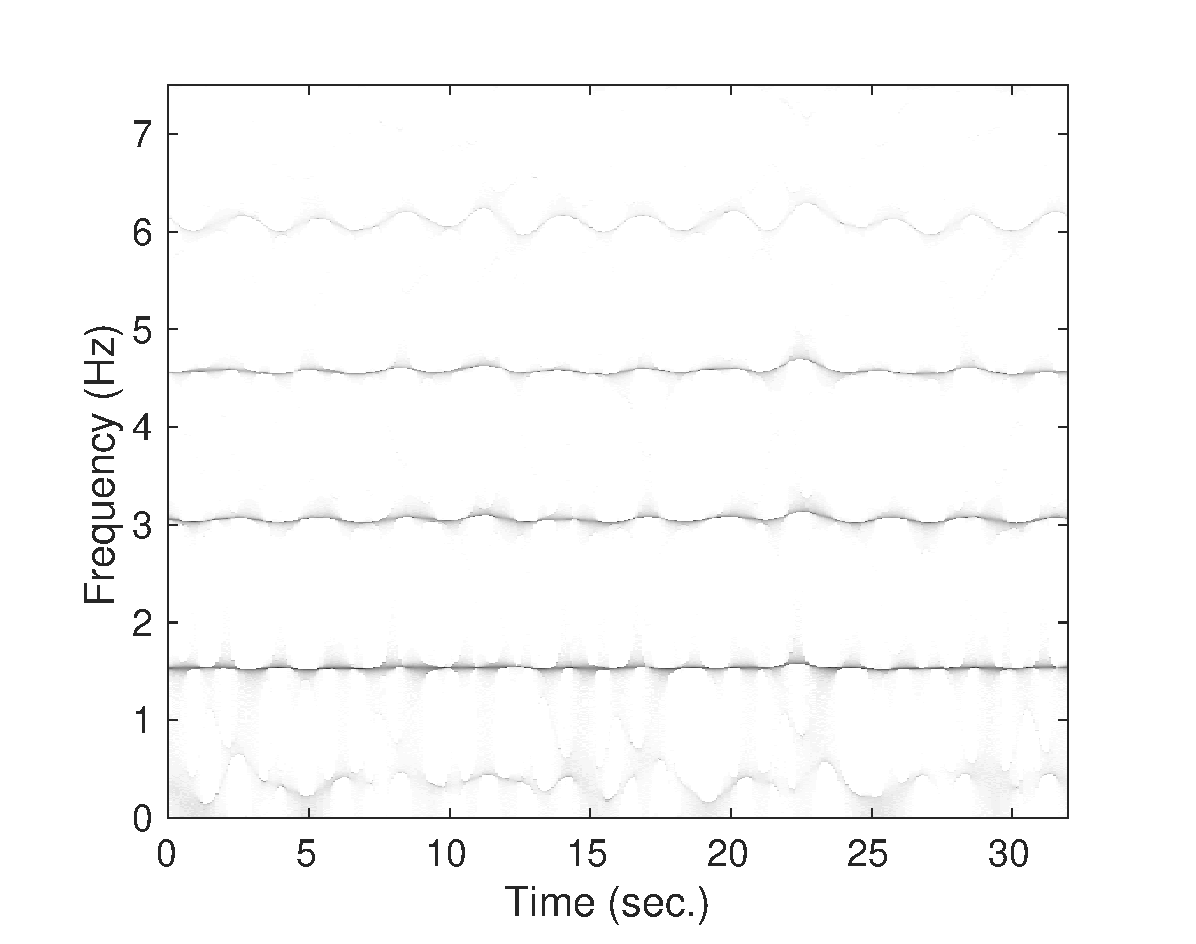
\includegraphics[width=.48\textwidth]{SSTBoundEffRed.eps}
%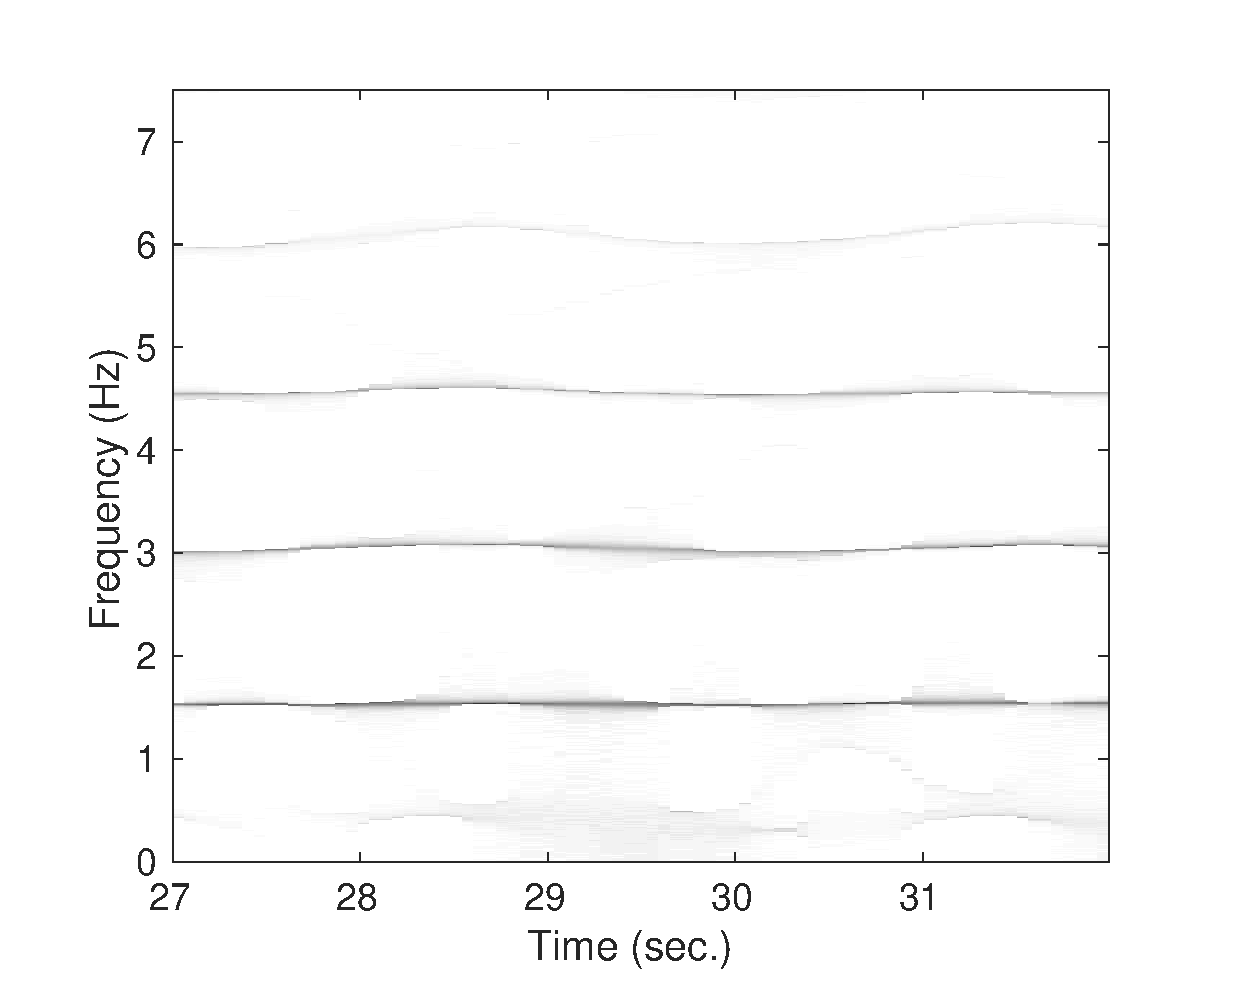
\includegraphics[width=.48\textwidth]{zoomSSTBoundEffRed.eps}
%\caption{Result of {\sf BoundEffRed} on the synchrosqueezing transform of a PPG (top) with a zoom on its right boundary (bottom). }
%\label{fig:ppg.boundeffred}
%\end{figure}


To evaluate the influence of the noise level on the performance of {\sf BoundEffRed}, we artificially add a Gaussian noise to the measured PPG signal. It is thus an additional noise to the measurement noise actually contained in the signal. Fig.~\ref{fig:otd.noise} shows the averaged OTD of {\sf BoundEffRed} for different values of the Signal to Noise Ratio (SNR). We notice that STFT is slightly more sensitive to noise than SST or RS, and STFT performs the best when the added noise is small, \ie~when the SNR is great. %On one hand, the robustness to noise of the SST and the RS is the direct consequence of the approximation result of~\cite{Daubechies16conceft}, discussed in section~\ref{sse:perf.BoundEffRed}. On the other hand, the sensitivity to noise of the STFT may be interpreted as the inability to forecast the values of the TF coefficients where only noise is active, while sharp TF representations, such as SST or RS, ideally vanish at these points.


\begin{figure}
\centering
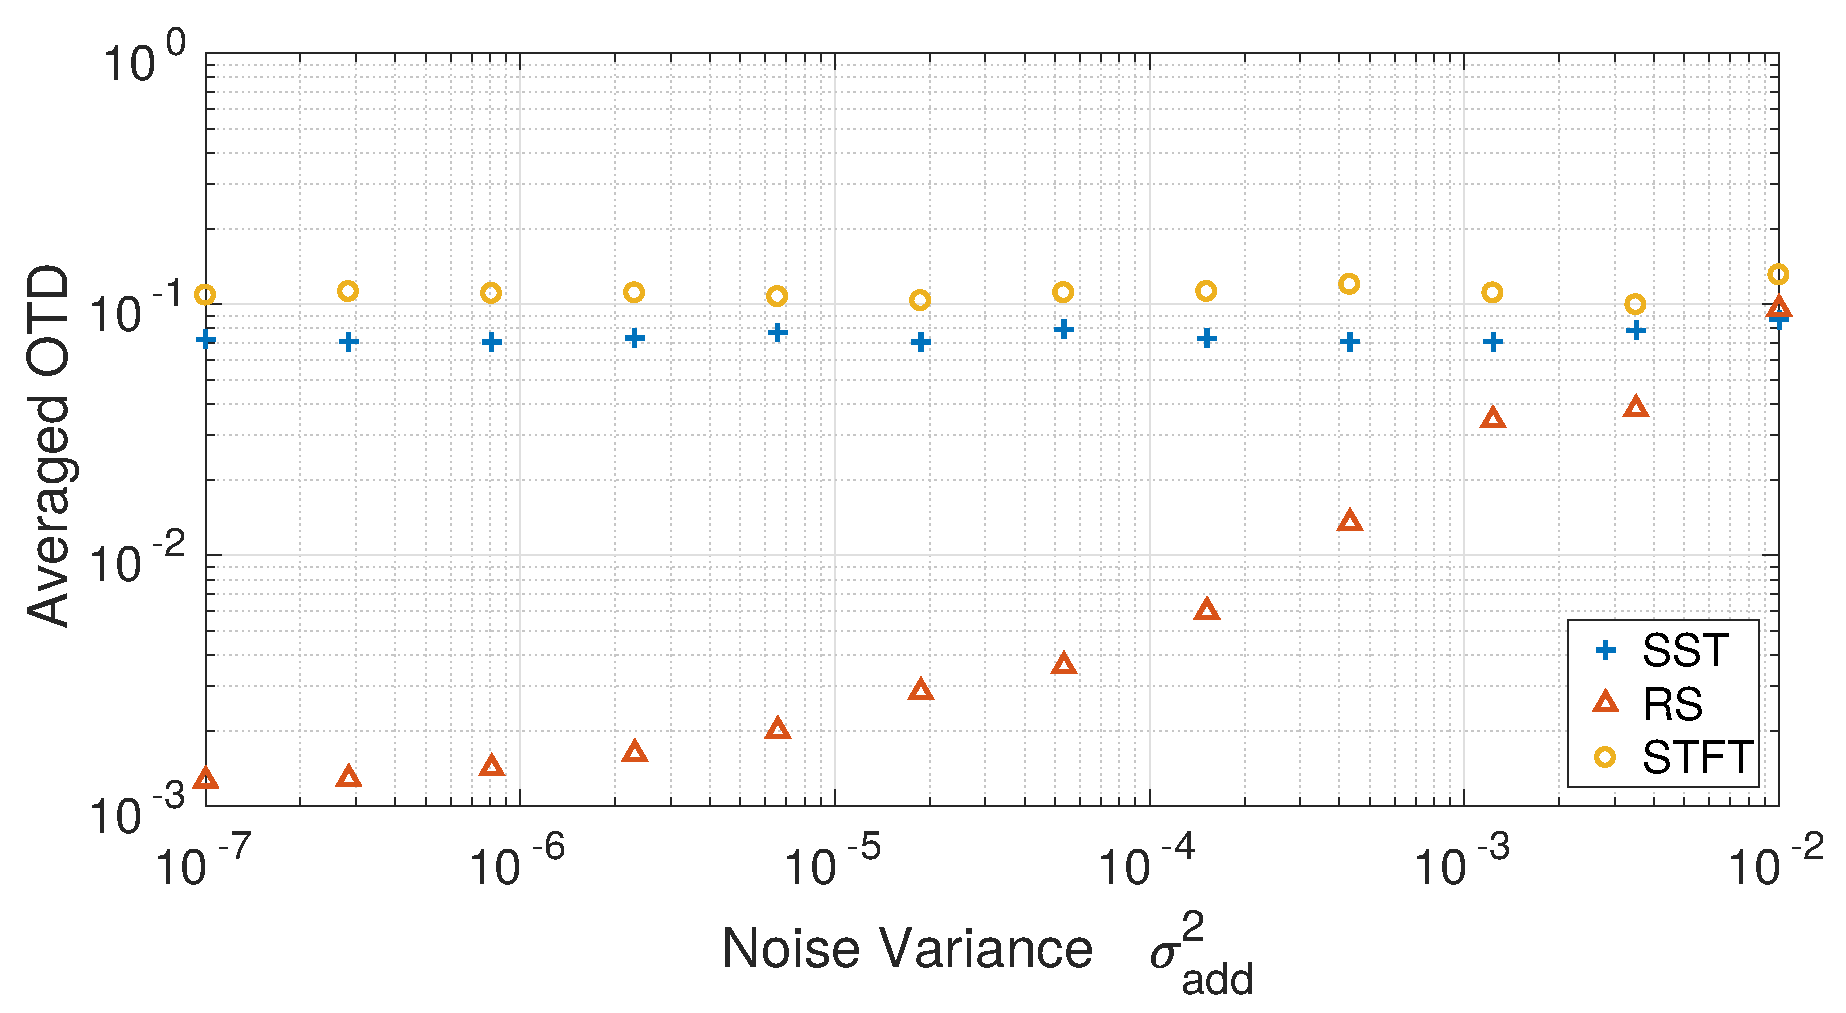
\includegraphics[width=.48\textwidth]{OTDBoundEffRed.eps}
\caption{PPG signal. Averaged OTD of {\sf BoundEffRed} in function of the SNR.}
\label{fig:otd.noise}
\end{figure} 